\section{Color Image}
Die Tristamlus Werte können von Rot (X), Grün (Y) und Blau (Z) berechnet werden. Da diese normalisiert sind, ergeben $x+y+z=1$
\[
x = \frac{X}{X+Y+Z} \quad 
y = \frac{Y}{X+Y+Z} \quad 
z = \frac{Z}{X+Y+Z} \quad 
\]
Damit kann das folgende Diagram erstellt werden
\begin{center}
	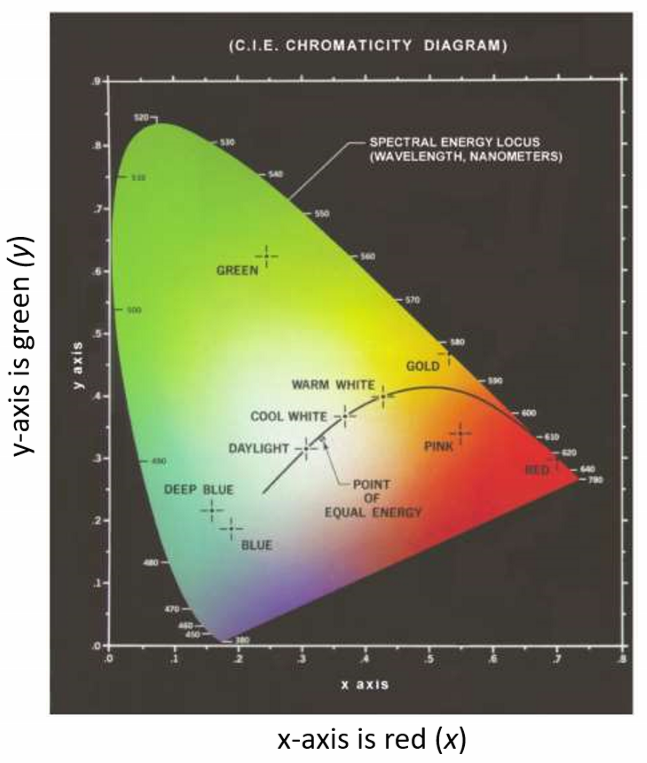
\includegraphics[width=\columnwidth]{Images/cie}
\end{center}

\subsection{RGB to CMY}
Mit normalisierten RGB Werden ergibt dies:
\[
\begin{pmatrix}
	C \\ M \\ Y
\end{pmatrix} = \begin{pmatrix}
1 \\ 1 \\ 1
\end{pmatrix} -  \begin{pmatrix}
R \\ G \\ B
\end{pmatrix}
\]

\subsection{HSI}
Das HSI Color Modell wird häufig in der Bildverarbeitung eingesetzt. Dabei stehen \textbf{H}ue für die Farbinformationen. Gegeben bei eine Winkel $\theta$, normalerweise $0^\circ$ bei der Roten-Achse. \textbf{S}aturation für die Länge zum Farbpunkt und \textbf{I}ntensität entspricht der Poition auf dr Verikalen Achse. HSI ist intuitiver für Bild Segmentation, wobei jedoch RGB die besseren Resultate liefert.
\[
H = \begin{cases}
	\theta & if B \le G \\
	360 - \theta & if B \gt G 
\end{cases}
\]


\[
\theta = \arccos\left[\frac{0.5(R- G) + (R-B)}{\sqrt{(R-G)^2 + (R-B)(G-B)}}\right]
\]

\[
S = 1 - \frac{3\cdot \min\{R,G,B\}}{R+G+B}
\]
\[
I = \frac{1}{3}(R+G+B)
\]

\subsection{Distances}
Um ein Objekt zu segmentieren, muss die ähnlichkeit von zwei Pixeln betrachtet werden. Dafür können Distanzen von $z$ zu $a$ berechnet werden.

\begin{align*}
	D(z,a) &= \begin{Vmatrix}z - a\end{Vmatrix} \\
	& = \sqrt{z-a)^T(z-a)} \\
	& = \sqrt{(z_R-a_R)^2+(z_G-a_G)^2+(z_B-a_B)^2}
\end{align*}

Eine andere Art Distanzen zu messen ist die Mahalanobis Distanz mit der Covariance Matrix $c$:
\[
D(z,a)=\sqrt{(z-a)^Tc^{-1}(z-a)}
\]